\documentclass{article}
%\usepackage{fullpage}
\usepackage{graphicx}
\usepackage{apacite}
\setlength{\parindent}{0pt}
\setlength{\parskip}{.3cm}
\title{Profile Analysis in \textbf{R} \\
{\normalsize version 1.0}}
\author{Christopher David Desjardins}
%\VignetteIndexEntry{An R Package for Profile Analysis}
\usepackage{Sweave}
\begin{document}

% Figures within a column...
\makeatletter
\newenvironment{tablehere}
{\def\@captype{table}}
{}
\newenvironment{figurehere}
{\def\@captype{figure}}
{}
\makeatother

\maketitle

The purpose of this manual is to document the \texttt{criterion.pattern()} and \texttt{profile.cv()} functions presented in
\citeA{davison2002identifying} and implemented in \textbf{R}. This manual begins with a brief introduction to reading data
into \textbf{R}, then describes the two principal functions and how to use them, and concludes with examples of both functions
that replicate the results presented in \citeA{davison2002identifying}. This manual assumes that the reader is familiar with this article. To more thoroughly understand these functions and their output, the reader should refer to that article.

Functions and arguments that can be sent to \textbf{R} are written in \texttt{this format} and libraries and
references to objects and output are written in \emph{this format}.

\section{Reading data into R}

 There are myriad ways that an applied researcher in education might want to read data into \textbf{R}. For the sake of simplicity, I will assume that a researcher is managing their data in \textbf{SPSS} and wants to read their data into \textbf{R}. There are two principal ways that this could be done. The first is directly through the \emph{foreign} library  and the \texttt{read.spss()} function. The second, indirectly, is by exporting ones' data from SPSS to a .csv file and then using the \texttt{read.csv()} function. I will demonstrate both ways.

\subsection{Reading SPSS data directly into \textbf{R} via the \emph{foreign} library.}

The \emph{foreign} library must be loaded initially and then the \texttt{read.spss()} function needs to be called.This library should be installed by default by \textbf{R}. If it is not, then it can be installed by running \texttt{install.packages("foreign")}.

\begin{Schunk}
\begin{Sinput}
> library(foreign)
> sack <- read.spss("sackett5.sav",to.data.frame=T,use.value.labels=T)
\end{Sinput}
\end{Schunk}

This assigns the sackett5.sav file to \emph{sack}, you are then able to directly manipulate the data file without needing to rerun
the \texttt{read.spss()} function again. The \texttt{head()} command shows the first few records in your data file so that you
can verify that the data was imported correctly.

\subsection{Reading SPSS data indirectly into \textbf{R} via the \texttt{read.csv()} function.}


To use this method it is assumed that you exported your data as a csv file in SPSS. This should be done in SPSS
and not in \textbf{R}.

\begin{Schunk}
\begin{Sinput}
> sack.csv <- read.csv(file = "sackett5.csv")
\end{Sinput}
\end{Schunk}

This assigns the sackett5.csv file to \emph{sack.csv} for later manipulation. After you have successfully read your data into \textbf{R} it is useful to save your data file in the native \textbf{R} file format, Rdata. To do this run the following:

\begin{Schunk}
\begin{Sinput}
> save(sack,file="sack.Rdata")
> load("sack.Rdata")
\end{Sinput}
\end{Schunk}

\section{Functions}
This section documents how to use the two principal functions, \texttt{criterion.pattern()} and
\texttt{profile.cv()}. In order to parallel nomenclature already presented in Davison and Davenport (2002), object names are
assigned the same names as those used by Davison and Davenport (2002) with the exception of a few objects.

\subsection{The criterion.pattern() function}

\begin{center} 
\texttt{criterion.pattern(x,y,k)} 
\end{center}

The \texttt{criterion.pattern()} function requires three arguments: \texttt{x}, \texttt{y}, and \texttt{k}. The argument
\texttt{x} corresponds to the predictor variables. This matrix of covariates may be in their own object or in the same object as the dependent variable. The \texttt{y} argument corresponds to the dependent variable. This vector may be in a separate object
or in the same object as \texttt{x}. Finally \texttt{k} corresponds to the scalar constant. It is necessary to supply the
\texttt{criterion.pattern()} function with these arguments.

\vspace{.2cm} 
As this function implements all of the algorithms described in Davison and Davenport (2002) with the exception of
the cross-validation (provided in \texttt{profile.cv()}) the output is contained within the function is quite exhaustive and the user should refer to that article for more information about how each specific component is calculated.

The default output from \texttt{criterion.pattern()} consists of three parts: The regression weights, the vector of regression weight deviations around the mean \emph{bstar}, the $R^2$ for the full model, for the level effect, and for the pattern effect. The default output also includes five F-test on these components: $H_o$: $R^2_{full} = 0$; $H_o$: $R^2_{pat} = 0$; $H_o$: $R^2_{lvl} = 0$; $H_o$: $R^2_{full} = R^2_{lvl}$; and $H_o$: $R^2_{full} = R^2_{pat}$. 

Additionally output may be called from the \texttt{criterion.pattern()}. This includes the level component (\emph{lvl.comp}) and the pattern component (\emph{pat.comp}). \emph{lvl.comp} provides a vector of scores corresponding to the level component. This is labeled as \textbf{X}$_p$ in \citeA{davison2002identifying}. \emph{pat.comp} provides the matrix of pattern component scores. This is labeled as \textbf{x}$_p$ in Davison and Davenport (2002). \emph{b} is a vector that contains the regression weights, this is not the deviation vector around the regression weight mean. The vector containing the regression weight deviations around the regression weight mean corresponds to \emph{bstar}. This is labeled b* in \citeA{davison2002identifying} but it is programmed as \emph{bstar} because \textbf{R} does not allow the use of the * key. \emph{xc} corresponds to the criterion pattern based on \emph{k} and can be calculated by multiplying \emph{bstar} and \emph{k}. The covariance between the actual predictor scores of person \textit{p} and their scores in criterion-pattern vector (\emph{Covpc)} is also available as is the vector of predicted scores, \emph{Ypred}. 

The examples below show how to run the functions, however, I recommend saving the output from the functions to an object so that you can easily retrieve them and in the case of \texttt{profile.cv()} so that results can be replicated. It is also necessary to store the output so that you can call the additional information available in the function.

\subsection{The profilecv() function}

\vspace{0.1cm} 
\begin{center} 
\texttt{profilecv(x,y)} 
\end{center}

\vspace{.1cm}

The \texttt{profilecv()} function implements the cross-validation technique described in \citeA{davison2002identifying}. It
requires two arguments: \texttt{x} and \texttt{y}. The argument \texttt{x} corresponds to the predictor variables. This matrix
of covariates may be in their own object or in the same object as the dependent variable. The \texttt{y} argument corresponds to the dependent variable. This vector may be in a separate object or in the same object as \texttt{x}. There is no \texttt{k}
argument for this function as \texttt{k} is irrelevant to this calculation.

\vspace{.2cm} There are five tables provided by this function: A F-table examining the full model, $H_o$:$R^2_{full} = 0$; a F-table examining the pattern effect, $H_o$: $R^2_{pat} = 0$; a F-table examining the level effect, $H_o$: $R^2_{lvl} = 0$; a F-table examining $H_o$: $R^2_{full} = R^2_{lvl}$; and a F-table examining $H_o$: $R^2_{full} = R^2_{pat}$. Within each of these table are estimates of the proportion of variance accounted for by the model/effect, the F-statistic, the degrees of freedom, and the p-values reported for each random sample. It should be noted that this function will never have the same output twice as each time \texttt{profile.cv()} is called, a new random split is made. If you want to get the same results it is necessary to use the \texttt{set.seed()} function.

Again, it is recommended that you save the output of this function to an object.

\section{Examples} 
To demonstrate the use of the \texttt{criterion.pattern()} and the \texttt{profilecv()} functions, two data
sets are provided. The first data set, labeled dd2002.Rdata, can be used to recreate table 1 in \citeA{davison2002identifying}.
The second data set, sack.Rdata, can be used to recreate example 1 using the Sackett data set. The Sackett data set is not in
the public domain and can not be shared.

\subsection{criterion.pattern()}


\subsubsection{criterion.pattern() IPMM example}
\begin{Schunk}
\begin{Sinput}
> ## Load the package
> library(profanal)
\end{Sinput}
\begin{Sinput}
> ## Results presented in Table 1 load("dd2002.Rdata")
> IPMMc <- matrix(c(75, 60, 50, 50, 60, 75, 45, 55, 60, 60, 55, 45, 50, 
           50, 75, 60, 45, 55, 60, 75, 55, 45, 60, 60),ncol=4,byrow=T)
> NP <- c(1,1,1,0,0,0)
> colnames(IPMMc) <- c("A","H","S","B")
> m0 <- criterion.pattern(IPMMc,NP,1)
> m0
\end{Sinput}
\begin{Soutput}
(Intercept)           A           H           S           B 
 0.50000000  0.00923077  0.02307692 -0.00923077 -0.02307692 
          A           H           S           B 
 0.00923077  0.02307692 -0.00923077 -0.02307692 
                 R2
Full Model 0.969231
Pattern    0.969231
Level      0.000000
               F.statistic df.1 df.2   pvalue
R2full = 0           7.875    4    1 0.260419
R2pat = 0           10.500    3    1 0.222190
R2lvl = 0            0.000    1    1 1.000000
R2full = R2lvl      10.500    3    1 0.222190
R2full = R2pat       0.000    1    1 1.000000
\end{Soutput}
\begin{Sinput}
> m1 <- criterion.pattern(IPMMc,NP,500)
\end{Sinput}
\end{Schunk}
Output from these functions are stored in \emph{m0} and \emph{m1}, respectively. Note that only the output from \emph{m0} is shown. The output from \emph{m1} can be easily called by typing \emph{m1} in the R-console. 

To evaluate what is in the \emph{m1} and examine the pattern component (\emph{pat.comp}).
\begin{Schunk}
\begin{Sinput}
> str(m1)
\end{Sinput}
\begin{Soutput}
List of 10
 $ lvl.comp: num [1:6] 58.8 58.8 55 58.8 58.8 ...
 $ pat.comp: num [1:6, 1:4] 16.25 1.25 5 -8.75 -13.75 ...
  ..- attr(*, "dimnames")=List of 2
  .. ..$ : NULL
  .. ..$ : chr [1:4] "A" "H" "S" "B"
 $ b       : Named num [1:5] 0.5 0.00923 0.02308 -0.00923 -0.02308
  ..- attr(*, "names")= chr [1:5] "(Intercept)" "A" "H" "S" ...
 $ bstar   : Named num [1:4] 0.00923 0.02308 -0.00923 -0.02308
  ..- attr(*, "names")= chr [1:4] "A" "H" "S" "B"
 $ xc      : Named num [1:4] 4.62 11.54 -4.62 -11.54
  ..- attr(*, "names")= chr [1:4] "A" "H" "S" "B"
 $ k       : num 500
 $ Covpc   : num [1:6, 1] 57.7 75 49 -57.7 -75 ...
 $ Ypred   : Named num [1:6] 0.9615 1.1 0.8923 0.0385 -0.1 ...
  ..- attr(*, "names")= chr [1:6] "1" "2" "3" "4" ...
 $ r2      : num [1:3, 1] 0.97 0.97 0
  ..- attr(*, "dimnames")=List of 2
  .. ..$ : chr [1:3] "Full Model" "Pattern" "Level"
  .. ..$ : chr "R2"
 $ F.table :'data.frame':	5 obs. of  3 variables:
  ..$ F.statistic: num [1:5] 7.88 10.5 0 10.5 0
  ..$ df         : num [1:5, 1:2] 4 3 1 3 1 1 1 1 1 1
  .. ..- attr(*, "dimnames")=List of 2
  .. .. ..$ : chr [1:5] "full.df" "pat.df" "lvl.df" "pat.df" ...
  .. .. ..$ : NULL
  ..$ pvalue     : num [1:5, 1] 0.26 0.222 1 0.222 1
  .. ..- attr(*, "dimnames")=List of 2
  .. .. ..$ : chr [1:5] "p.value.F.R2.full" "p.value.F.R2.pat.only" "p.value.F.R2.lvl.only" "p.value.F.R2.pat" ...
  .. .. ..$ : NULL
 - attr(*, "class")= chr "critpat"
\end{Soutput}
\begin{Sinput}
> m1$pat.comp
\end{Sinput}
\begin{Soutput}
          A      H      S      B
[1,]  16.25   1.25  -8.75  -8.75
[2,]   1.25  16.25 -13.75  -3.75
[3,]   5.00   5.00   0.00 -10.00
[4,]  -8.75  -8.75  16.25   1.25
[5,] -13.75  -3.75   1.25  16.25
[6,]   0.00 -10.00   5.00   5.00
\end{Soutput}
\end{Schunk}

To replicate the Figure 1 in \citeA{davison2002identifying}

\begin{Schunk}
\begin{Sinput}
> m2 <- criterion.pattern(IPMMc,NP,1000)
> plot(m2$xc, type="b",ylab="Criterion Pattern Score")
> abline(a=0,b=0)
> text(m2$xc,labels(m2$xc), cex=1, pos=3)
\end{Sinput}
\end{Schunk}

\begin{figurehere}
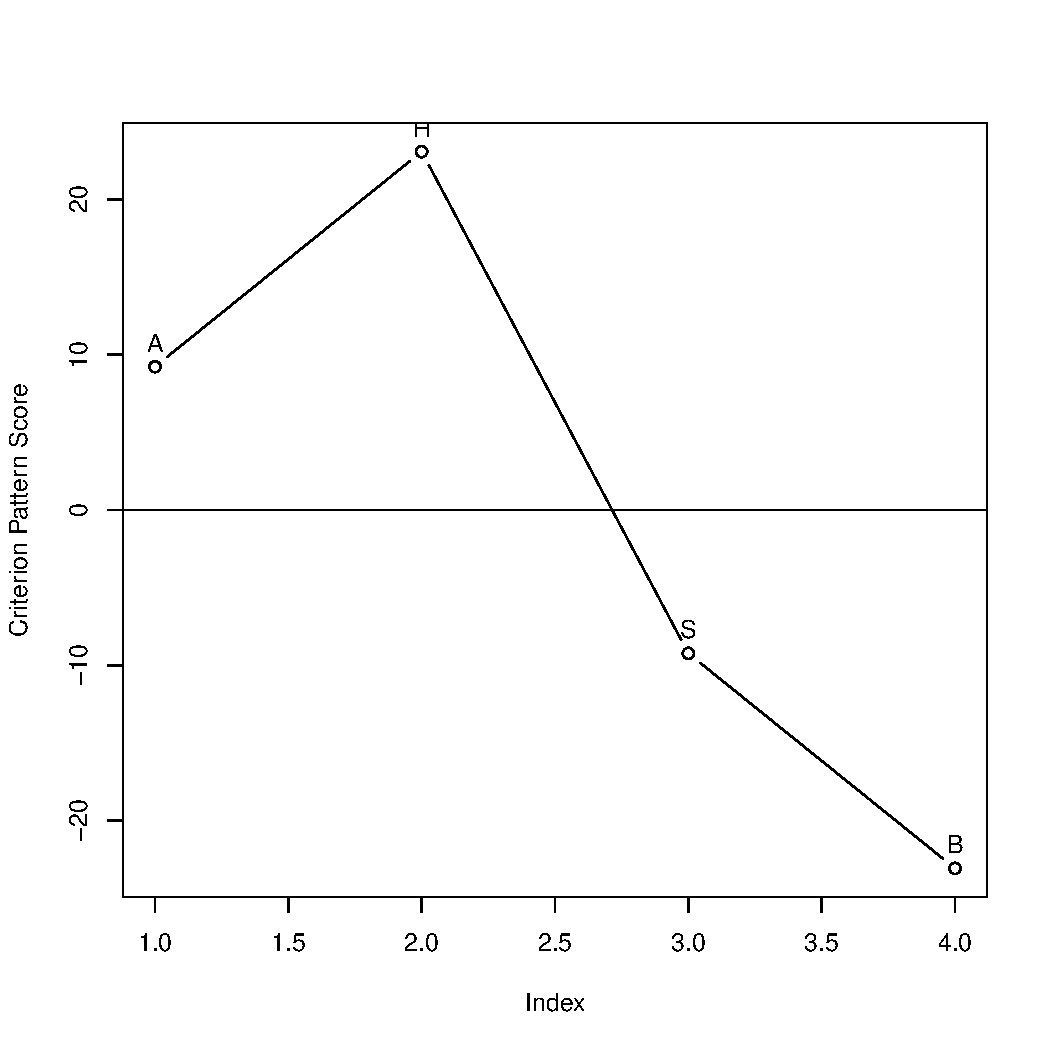
\includegraphics{fig1.pdf}
\end{figurehere}

\subsubsection{criterion.pattern() Sackett example}
\begin{Schunk}
\begin{Sinput}
## Unfortunately not available to share but include to reproduce Davison & Davenport (2002)'s findings.
> load("sack.Rdata")
> sack.m <- na.omit(sack)
> criterion.pattern(x = as.matrix(sack.m[, 2:7]), y = as.matrix(sack.m[, 
+     1]), k = 100)
\end{Sinput}
\begin{Soutput}
 (Intercept)       rtheme       itheme       atheme       stheme       etheme 
41.449243157 -0.211675068  0.009353870 -0.005280127  0.308281646  0.103993332 
      ctheme 
-0.083369241 
     rtheme      itheme      atheme      stheme      etheme      ctheme 
-0.23189247 -0.01086353 -0.02549753  0.28806424  0.08377593 -0.10358664 
                 R2
Full Model 0.133327
Pattern    0.129174
Level      0.006036
               F.statistic df.1 df.2   pvalue
R2full = 0        8.230315    6  321 0.000000
R2pat = 0         9.523090    5  321 0.000000
R2lvl = 0         1.949263    1  321 0.163631
R2full = R2lvl    9.429267    5  321 0.000000
R2full = R2pat    1.538263    1  321 0.215782
\end{Soutput}
\end{Schunk}
Th
e \texttt{as.matrix()} command is necessary as \texttt{X} and \texttt{Y} are in the same object. Therefore, I am assigning
column vectors 2 through 7 to \texttt{X} and column vector 1 to \texttt{Y}. In the first example, \emph{m0}, you can see that
the predictor variables and the dependent variable are stored in different objects. In both examples, \texttt{k} is assigned on
the fly.

As shown in the first example, \texttt{criterion.pattern()} will assume that the first argument you give is for \texttt{X}, the
next for \texttt{Y}, and the final argument for \texttt{k}. You do not have to specify these arguments in this order but if you
do not specify them in this order then you need to use \texttt{X=} and so on.

\subsection{criterion.pattern()}
\begin{Schunk}
\begin{Sinput}
> source("criterion_pattern-0.1.R")
> c0 <-profilecv(x=as.matrix(sack.m[,2:7]),y=as.matrix(sack.m[,1]))
> c0
\end{Sinput}
\begin{Soutput}
$R2.full
                      R2 F.statistic df1 df2   pvalue
Random Sample 1 0.129565    23.96501   1 161 0.000002
Random Sample 2 0.077396    13.50603   1 161 0.000323

$R2.pat
                      R2 F.statistic df1 df2   pvalue
Random Sample 1 0.127511    23.67578   1 162 0.000003
Random Sample 2 0.073950    12.93650   1 162 0.000428

$R2.lvl
                      R2 F.statistic df1 df2   pvalue
Random Sample 1 0.004617    0.751455   1 162 0.387298
Random Sample 2 0.004861    0.791322   1 162 0.375020

$R2.full.lvl
                      R2 F.statistic df1 df2   pvalue
Random Sample 1 0.127511    23.25453   1 162 0.000003
Random Sample 2 0.073950    12.73638   1 162 0.000472

$R2.full.pat
                      R2 F.statistic df1 df2   pvalue
Random Sample 1 0.004617    0.382216   1 162 0.537288
Random Sample 2 0.004861    0.605098   1 162 0.437774
\end{Soutput}
\end{Schunk}

\section{Additional output from \texttt{criterion.pattern()}}

\begin{Schunk}
\begin{Sinput}
> m1$lvl.comp
\end{Sinput}
\begin{Soutput}
[1] 58.75 58.75 55.00 58.75 58.75 55.00
\end{Soutput}
\begin{Sinput}
> m1$pat.comp
\end{Sinput}
\begin{Soutput}
          A      H      S      B
[1,]  16.25   1.25  -8.75  -8.75
[2,]   1.25  16.25 -13.75  -3.75
[3,]   5.00   5.00   0.00 -10.00
[4,]  -8.75  -8.75  16.25   1.25
[5,] -13.75  -3.75   1.25  16.25
[6,]   0.00 -10.00   5.00   5.00
\end{Soutput}
\begin{Sinput}
> m1$b
\end{Sinput}
\begin{Soutput}
(Intercept)           A           H           S           B 
 0.50000000  0.00923077  0.02307692 -0.00923077 -0.02307692 
\end{Soutput}
\begin{Sinput}
> m1$bstar
\end{Sinput}
\begin{Soutput}
          A           H           S           B 
 0.00923077  0.02307692 -0.00923077 -0.02307692 
\end{Soutput}
\begin{Sinput}
> m1$xc
\end{Sinput}
\begin{Soutput}
         A          H          S          B 
  4.615385  11.538462  -4.615385 -11.538462 
\end{Soutput}
\begin{Sinput}
> m1$k
\end{Sinput}
\begin{Soutput}
[1] 500
\end{Soutput}
\begin{Sinput}
> m1$Covpc
\end{Sinput}
\begin{Soutput}
          [,1]
[1,]  57.69231
[2,]  75.00000
[3,]  49.03846
[4,] -57.69231
[5,] -75.00000
[6,] -49.03846
\end{Soutput}
\begin{Sinput}
> m1$Ypred
\end{Sinput}
\begin{Soutput}
          1           2           3           4           5           6 
 0.96153846  1.10000000  0.89230769  0.03846154 -0.10000000  0.10769231 
\end{Soutput}
\begin{Sinput}
> m1$r2
\end{Sinput}
\begin{Soutput}
                 R2
Full Model 0.969231
Pattern    0.969231
Level      0.000000
\end{Soutput}
\begin{Sinput}
> m1$F.table
\end{Sinput}
\begin{Soutput}
               F.statistic df.1 df.2   pvalue
R2full = 0           7.875    4    1 0.260419
R2pat = 0           10.500    3    1 0.222190
R2lvl = 0            0.000    1    1 1.000000
R2full = R2lvl      10.500    3    1 0.222190
R2full = R2pat       0.000    1    1 1.000000
\end{Soutput}
\end{Schunk}

\bibliographystyle{apacite}
\bibliography{profanalnotes}


\end{document}
